\documentclass[12pt,a4paper,twoside]{report}
\usepackage{arabtex}
\usepackage[utf8]{inputenc}
\usepackage[T1]{fontenc}
\usepackage{fancyhdr}

\usepackage{lastpage}
\usepackage{a4wide} 
\usepackage{amsmath}

\usepackage{array}
\usepackage{multirow}
\usepackage{titlesec}
\usepackage{enumitem}


\newenvironment{thewebography}[1]
     {\section*{Sites et internets}%
      \list{\@biblabel{\@arabic\c@enumiv}}%
           {\settowidth\labelwidth{\@biblabel{#1}}%
            \leftmargin\labelwidth
            \advance\leftmargin\labelsep
            \@openbib@code
            \usecounter{enumiv}%
            \let\p@enumiv\@empty
            \renewcommand\theenumiv{\@arabic\c@enumiv}}%
      \sloppy
      \clubpenalty4000
      \@clubpenalty \clubpenalty
      \widowpenalty4000%
      \sfcode`\.\@m}
     {\def\@noitemerr
       {\@latex@warning{Empty `thewebography' environment}}%
      \endlist}
\makeatother

\titlespacing{\subsubsection}{0pt}{\parskip}{-\parskip}
\raggedbottom

\usepackage{amssymb} 
\usepackage{graphicx}
\usepackage{color}
\usepackage{fancybox}
\usepackage{moreverb}
\usepackage[english,francais]{babel}
\usepackage{listings}
\PassOptionsToPackage{hyphens}{url}\usepackage{hyperref}
\usepackage{lscape}
\usepackage[footnote]{acronym}
\usepackage{textcomp}
\usepackage{longtable}
\usepackage{titlesec}


\usepackage{float}

\usepackage{nomencl}
\usepackage[titletoc]{appendix}

\makenomenclature

\usepackage{amsmath,amsfonts}

\renewcommand{\labelitemii}{$\star$}

\usepackage{geometry}
\geometry{hmargin=2.5cm,vmargin=2.5cm}

\newcommand\x{13cm}

\setlength{\parskip}{0em}

\setcounter{tocdepth}{4}
\setcounter{secnumdepth}{4}
\renewcommand{\baselinestretch}{1.5}
\makeatletter
\renewcommand\@bibitem[1]{\item\if@filesw \immediate\write\@auxout
    {\string\bibcite{#1}{W\the\value{\@listctr}}}\fi\ignorespaces}% <------------



\pagestyle{fancy}
\fancyhf{}
\fancyhead[RE,RO]{\leftmark}
\fancyfoot[RE,LO]{UM5R}
\fancyfoot[LE,RO]{ENSIAS}
\fancyfoot[CE,CO]{\thepage}
\renewcommand{\headrulewidth}{2pt}
\renewcommand{\footrulewidth}{1pt}
\usepackage{hyperref}
\usepackage{wrapfig}
\titlespacing{\subsection} {4ex} {*0} {*0} {}   
\titlespacing{\subsubsection} {8ex} {*0} {*0} {}   


%Options: Sonny, Lenny, Glenn, Conny, Rejne, Bjarne, Bjornstrup
\usepackage[Glenn]{fncychap}

\begin{document}
	\thispagestyle{empty}
	\makeatother
	\title{rapport de stage de 1ere annee}
	\author{EL YOUSSR Mohamed Amine}
	\date{\today}


	\lstset{ numbers=left, tabsize=3, frame=single, numberstyle=\ttfamily, basicstyle=\footnotesize} 
	%%%%%%%%%%%%%%
	%page de garde
	%%%%%%%%%%%%%%
	\begin{minipage}[l]{.10\linewidth}
			\begin{center}
				
\includegraphics[width=4cm]{Images/logo/ensias.png}
			\end{center}
	\end{minipage} \hfill
	\begin{minipage}[r]{.36\linewidth}
			\begin{center}
				
\includegraphics[width=4cm]{Images/logo/um5.png}
			\end{center}
	\end{minipage}
	
	\vspace{1.5cm}
	
	\begin{center}
			{\LARGE \textbf{Rapport du Projet JEE }}\\
			\textbf{Filère : Génie logiciel}
			\vspace{2cm}

			% Title
			\rule{\linewidth}{0.6mm} \\[0.5cm]
				{ \huge \bfseries Application Web pour l'automatisation du prossesus de don du sang \\[0.4cm] }
			\rule{\linewidth}{0.6mm} \\[1cm]

			\vspace{2cm}

			% Author and supervisor
			\noindent
			\begin{minipage}[t]{.60\textwidth}
					\large
							\emph{\textbf{Réalisé par :}} \\
							EL YOUSSR Mohamed Amine\\
							 MOSSATI Oussama\\
							 EL MAHDI Zouhair\\
							 MEJDAOUI Soufiane\\
							
					
			\end{minipage}
			\begin{minipage}[t]{.30\textwidth}
						
							\emph{\textbf{Encadré par :}}\\
							 ELHAMLAOUI Mahmoud\\
						
			\end{minipage}

			\vfill

			\vspace{1.5cm}
			{\large Année Universitaire: 2019 - 2020 }
	\end{center}

	\newpage
	\thispagestyle{empty}
	\setcounter{page}{1}
	\vspace*{\stretch{1}}
		
	
	\newpage
		
	\addcontentsline{toc}{chapter}{Table des figures}
				\listoffigures
		
		\newpage
			

	\printnomenclature

	\begingroup
\makeatletter

\tableofcontents{}

\endgroup
	
	\newpage

	\chapter*{Introduction générale}
	\addcontentsline{toc}{chapter}{Introduction générale}
	\markboth{INTRODUCTION GÉNÉRALE}{INTRODUCTION GÉNÉRALE}
	\label{chap:introduction}{
		Après avoir terminer le cours de l'élément du module "Ingénieurie Web", on était amené à réaliser un projet pour appliquer les connaissances aquises dans de cet élément.\\
		Pour notre cas, on a choisit un sujet qui peut s'appliquer dans le domaine de la santé et spécifiquement "Le don du sang". Il s'agit de développer une application Web en langage JEE qui permet l'automatisation du processus du don du sang.\\
		L'application développée aura comme objectif principale la diffision des informations surtout dans le cas des besoins urgents (soit par Mail, par SMS et par Twitter), Consultation des statisques, Interaction avec un Chatbot et d'autres fonctionnalités.\\
		Ce document présente les différentes phase de développement du projet qui s"'est déroulé en semaines.\\
		On commence par l'analyse des différents besoins, et la conception de la solution. Ensuite, on va aborder le choix des technologies et la présentation de l'application sous forme des captures d'écrans.

	 }
		
	\newpage
	
	\chapter{Analyse \& Conception}{
		Une fois la problématique est posée, l’étape suivante est l’étude de l’existant, l’analyse des besoins et la conception de la solution qui va mener à la réussite du projet.
	\newpage
	}
	\section{Analyse des besoins :}{
			\subsection{Besoins fonctionnels :}{
				Il s’agit des fonctionnalités à assurer par le futur logiciel. Ce sont les besoins spécifiant le comportement d’entrée/ sortie. L’application doit permettre de :
				\begin{itemize}[label=\textbullet]
				\item \textbf{Gérer l’authentification :} Pour l’accès aux espaces basé sur role de l’utilisateur (généralement, on a 3 roles : Administrateur,Responsable de la banque du sang et Donateur).
				\item \textbf{Pour l'administrateur ,} il peut :
						\begin{itemize}
							\item Gérer des banques de sang.
							\item Gérer des donateurs.
							\item Consulter les convois.
							\item Consulter les alertes des besoins.
							\item Consulter les statistiques des banques de sang.
						\end{itemize}
				\item \textbf{Pour le responsable de la banque du sang,} il peut :
						\begin{itemize}
								\item Gérer les alertes des besoins.
								\item Gérer les convois et leurs plannings.
								\item Gérer les donations.
								\item Gérer le stock du sang.
								\item Consulter les statistiques.
						\end{itemize}
				\item \textbf{Pour le donateur :}
						\begin{itemize}
								\item Consulter ses donations.
								\item Consulter les alertes des besoins.
								\item Consulter les convois.
						\end{itemize}
			\end{itemize}
			}
			\subsection{Besoins non fonctionnels :}{
				Il s’agit des fonctionnalités qui caractérisent le système. Ce sont des besoins liés à la performance et le type de conception. Ces besoins peuvent concerner les contraintes d’implémentation (langage de programmation, type SGBD, de système d'Exploitation...). Le futur logiciel doit nécessairement assurer ces besoins :
				\begin{itemize}[label=$\Diamond$]
						\item \textbf{Compatibilité :} l'application doit être compatible avec des applications partagées, avec des applications tierces, sur des systèmes d’exploitation et des plateformes différents.
						\item \textbf{Extensibilité :} l'application devra être extensible, c'est à dire qu'il pourra y avoir une possibilité d'ajouter ou de modifier de nouvelles fonctionnalités.
						\item \textbf{Performance :} l’application devra être performante, c'est-à-dire que le système doit réagir dans un délai précis, quel que soit l’action de l’utilisateur.
						\item \textbf{Fiabilité :} le système doit garantir la rapidité et la fiabilité de la recherche des informations, ainsi qu'une gestion optimale des ressources.
						\item \textbf{Convivialité :} l’application doit être simple et facile à manipuler même par des non experts.
						\item \textbf{Sécurité :} l’application devra être hautement sécurisée, les informations ne devront pas être accessibles à tout le monde, c'est-à-dire que l'application est accessible par un identifiant et un mot de passe attribué à une personne physique.
				\end{itemize}
			}
	}
	\section{Conception :}{
		
			\subsection{Diagramme des cas d'utilisations :}{
				Afin de donner une vision globale du comportement fonctionnel du système, on présente ci-dessous le diagrammes des cas d’utilisations.
								\begin{figure}[H]
									 \includegraphics[width=13cm]{Images/usecase.png}
									 \centering
									 \caption{\label{usd1} Diagramme de cas d'utilisations}
								\end{figure}
						
			}
	
		\subsection{Diagramme de classe:}{
			Le diagramme de classes est considéré le plus important de la modélisation orientée objet. Il montre la structure interne du système et permet de fournir une représentation abstraite des objets du système qui vont interagir ensemble pour réaliser les cas d’utilisation.
				\begin{figure}[H]
					 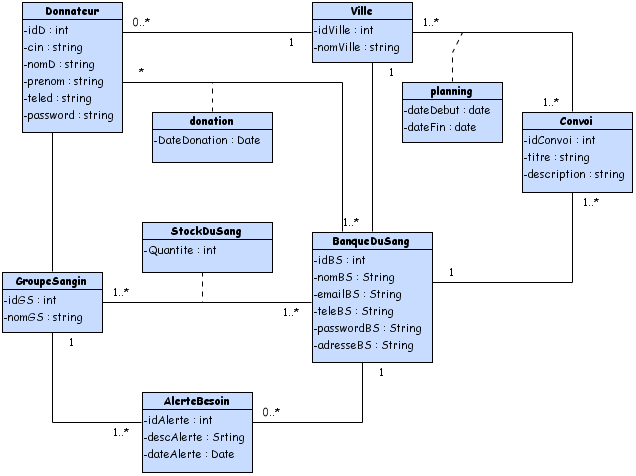
\includegraphics[width=15cm]{Images/class.png}
					 \centering
					 \caption{\label{classe} Diagramme de classe}
				\end{figure}
		}
	}
	
	\newpage
	
	\chapter{Etude technique \& Réalisation}{
		Après avoir exprimé les différentes fonctionnalités envisagées par l’application, ainsi que sa conception, On va présenter dans ce chapitre l’architecture technique du projet et les outils et Framework de développement, ainsi que la réalisation informatique de ses composantes. Il s’agit de la mise en oeuvre des principales fonctions proposées pour tester le fonctionnement du l’application.
	\newpage
	}
	\section{Choix des outils \& technologies :}{
			\begin{itemize}[label=\textbullet]
				\item Langage de programmation: Java/JEE.
				\item Servlets/JSP/JSTL.
				\item Serveur d'application: Tomcat Server.
				\item Maven.
				\item SGBD: MySQL.
				\item Gestion des versions: Git/GitHub.
				\item Envoi des MAILs : API javax.mail.
				\item Envoi des SMSs : API nexmo.
				\item Publication sur Twitter : API Twitter4J.
				\item Traitement asynchrone : AJAX.
				\item ChatBot : DialogFlow.
				\item Design: Bootstrap4.
			\end{itemize}
	}
	\section{Présentation de l'application :}{
	}
	\chapter*{Conclusion \& Percpectives}
	\addcontentsline{toc}{chapter}{Conclusion \& Percpectives}
	\markboth{CONCLUSION \& PERCPECTIVES}{CONCLUSION \& PERCPECTIVES}
	\label{chap:conclusion}{
		Ce rapport présente brièvement le projet que nous étions amené à le réaliser durant 3 semaines. Pour mettre en oeuvre ce projet, on a établi dans un premier lieu
une analyse des diffrents besoins suivie par une étude conceptuelle du sujet affin de dégager les différents fonctionnalités du système ainsi qu'une étude des outils et technologies qui seront utilisés pour la réalisation de l'application.

On a essayé au maximum de respecter les fonctionnalités établies dans la phase d'analyse.

Sur le plan personnel, ce projet était pour nous une opportunité et une expérience très satisfaisante et enrichissante, grâce à ce projet on a appris et on a approfondis des connaissances sur des nouvelles technologies.

Comme perspectives de ce travail, on a voulu ajouter des nouvelles fonctionnalités comme l’échange des messages entre les différentes entité du système par les websockets, et on a voulu aussi entamer une partie très importante qui est la partie des tests (Dans notre cas, c'était avec l'outil JUnit) et la partie de de déploiment (DOCKER), mais suite à des contraintes de temps, on a pas pu les faire.

En somme ce projet nous a permis de mettre en pratique et d'approfondir les connaissances reçues au cours enseignés à l'École nationale supérieure d'informatique et d'analyse des systèmes. Ce projet s'est très bien déroulé, et a été pour nous une véritable opportunité d'apprendre, de découvrir et d'être plus efficace.
	}

\renewcommand{\bibname}{Bibliographie et Webographie}
\begin{thebibliography}{3}
	\bibliographystyle{alpha}
	\addcontentsline{toc}{chapter}{Bibliographie et Webographie}

	\bibitem{jee}[En ligne] (JEE) Disponible sur :
	\\\texttt{https://docs.oracle.com/javaee/}

	\bibitem{intellij}[En ligne] (intellij) Disponible sur :
	\\\texttt{https://fr.wikipedia.org/wiki/IntelliJ\_IDEA}

	\bibitem{maven}[En ligne] (maven) Disponible sur :
	\\\texttt{https://fr.wikipedia.org/wiki/Apache\_Maven}

	\bibitem{git}[En ligne] (git) Disponible sur :
	\\\texttt{https://fr.wikipedia.org/wiki/Git}

	\bibitem{github}[En ligne] (github) Disponible sur :
	\\\texttt{https://fr.wikipedia.org/wiki/GitHub}
\end{thebibliography}
\end{document}
